GEANT4 is a free toolkit for the simulation of particles as they travel through matter\cite{agostinelli_geant4simulation_2003}.
In general two types of applications were authored with the GEANT4 toolkit; ranges along with energy deposition and light transport.
All of the applications shared a common electromagnetic physics list based on the Livermore data set, and a cross section driven hadron physics list was used for the neutron interactions.
Ions were transported with the general ion physics list which contains detailed alpha and triton models.
Optical photons were transported with the default Optical Photon physics list.
More details on the GEANT4 toolkit may be found in \autoref{chap:G4Intro}.

\subsection{Energy Deposition Simulations}
\label{sec:EnergyDeposition}
The GEANT4 toolkit has the ability to track the energy deposition in different materials as well as the tracking of electrons to a least \SI{1}{\keV}\cite{agostinelli_geant4simulation_2003}.
It is proposed to represent the detector geometry as a single layer of neutron absorbing thin polymeric film mounted on top of a non-scintillating material (PMMA).
For simplicity, the initial events for runs will be chosen by setting up a particle gun for thermal (\SI{0.025}{\eV}) neutrons upon the detector and for both gammas resulting from a \iso[60]{Co} decay.
\begin{figure}
  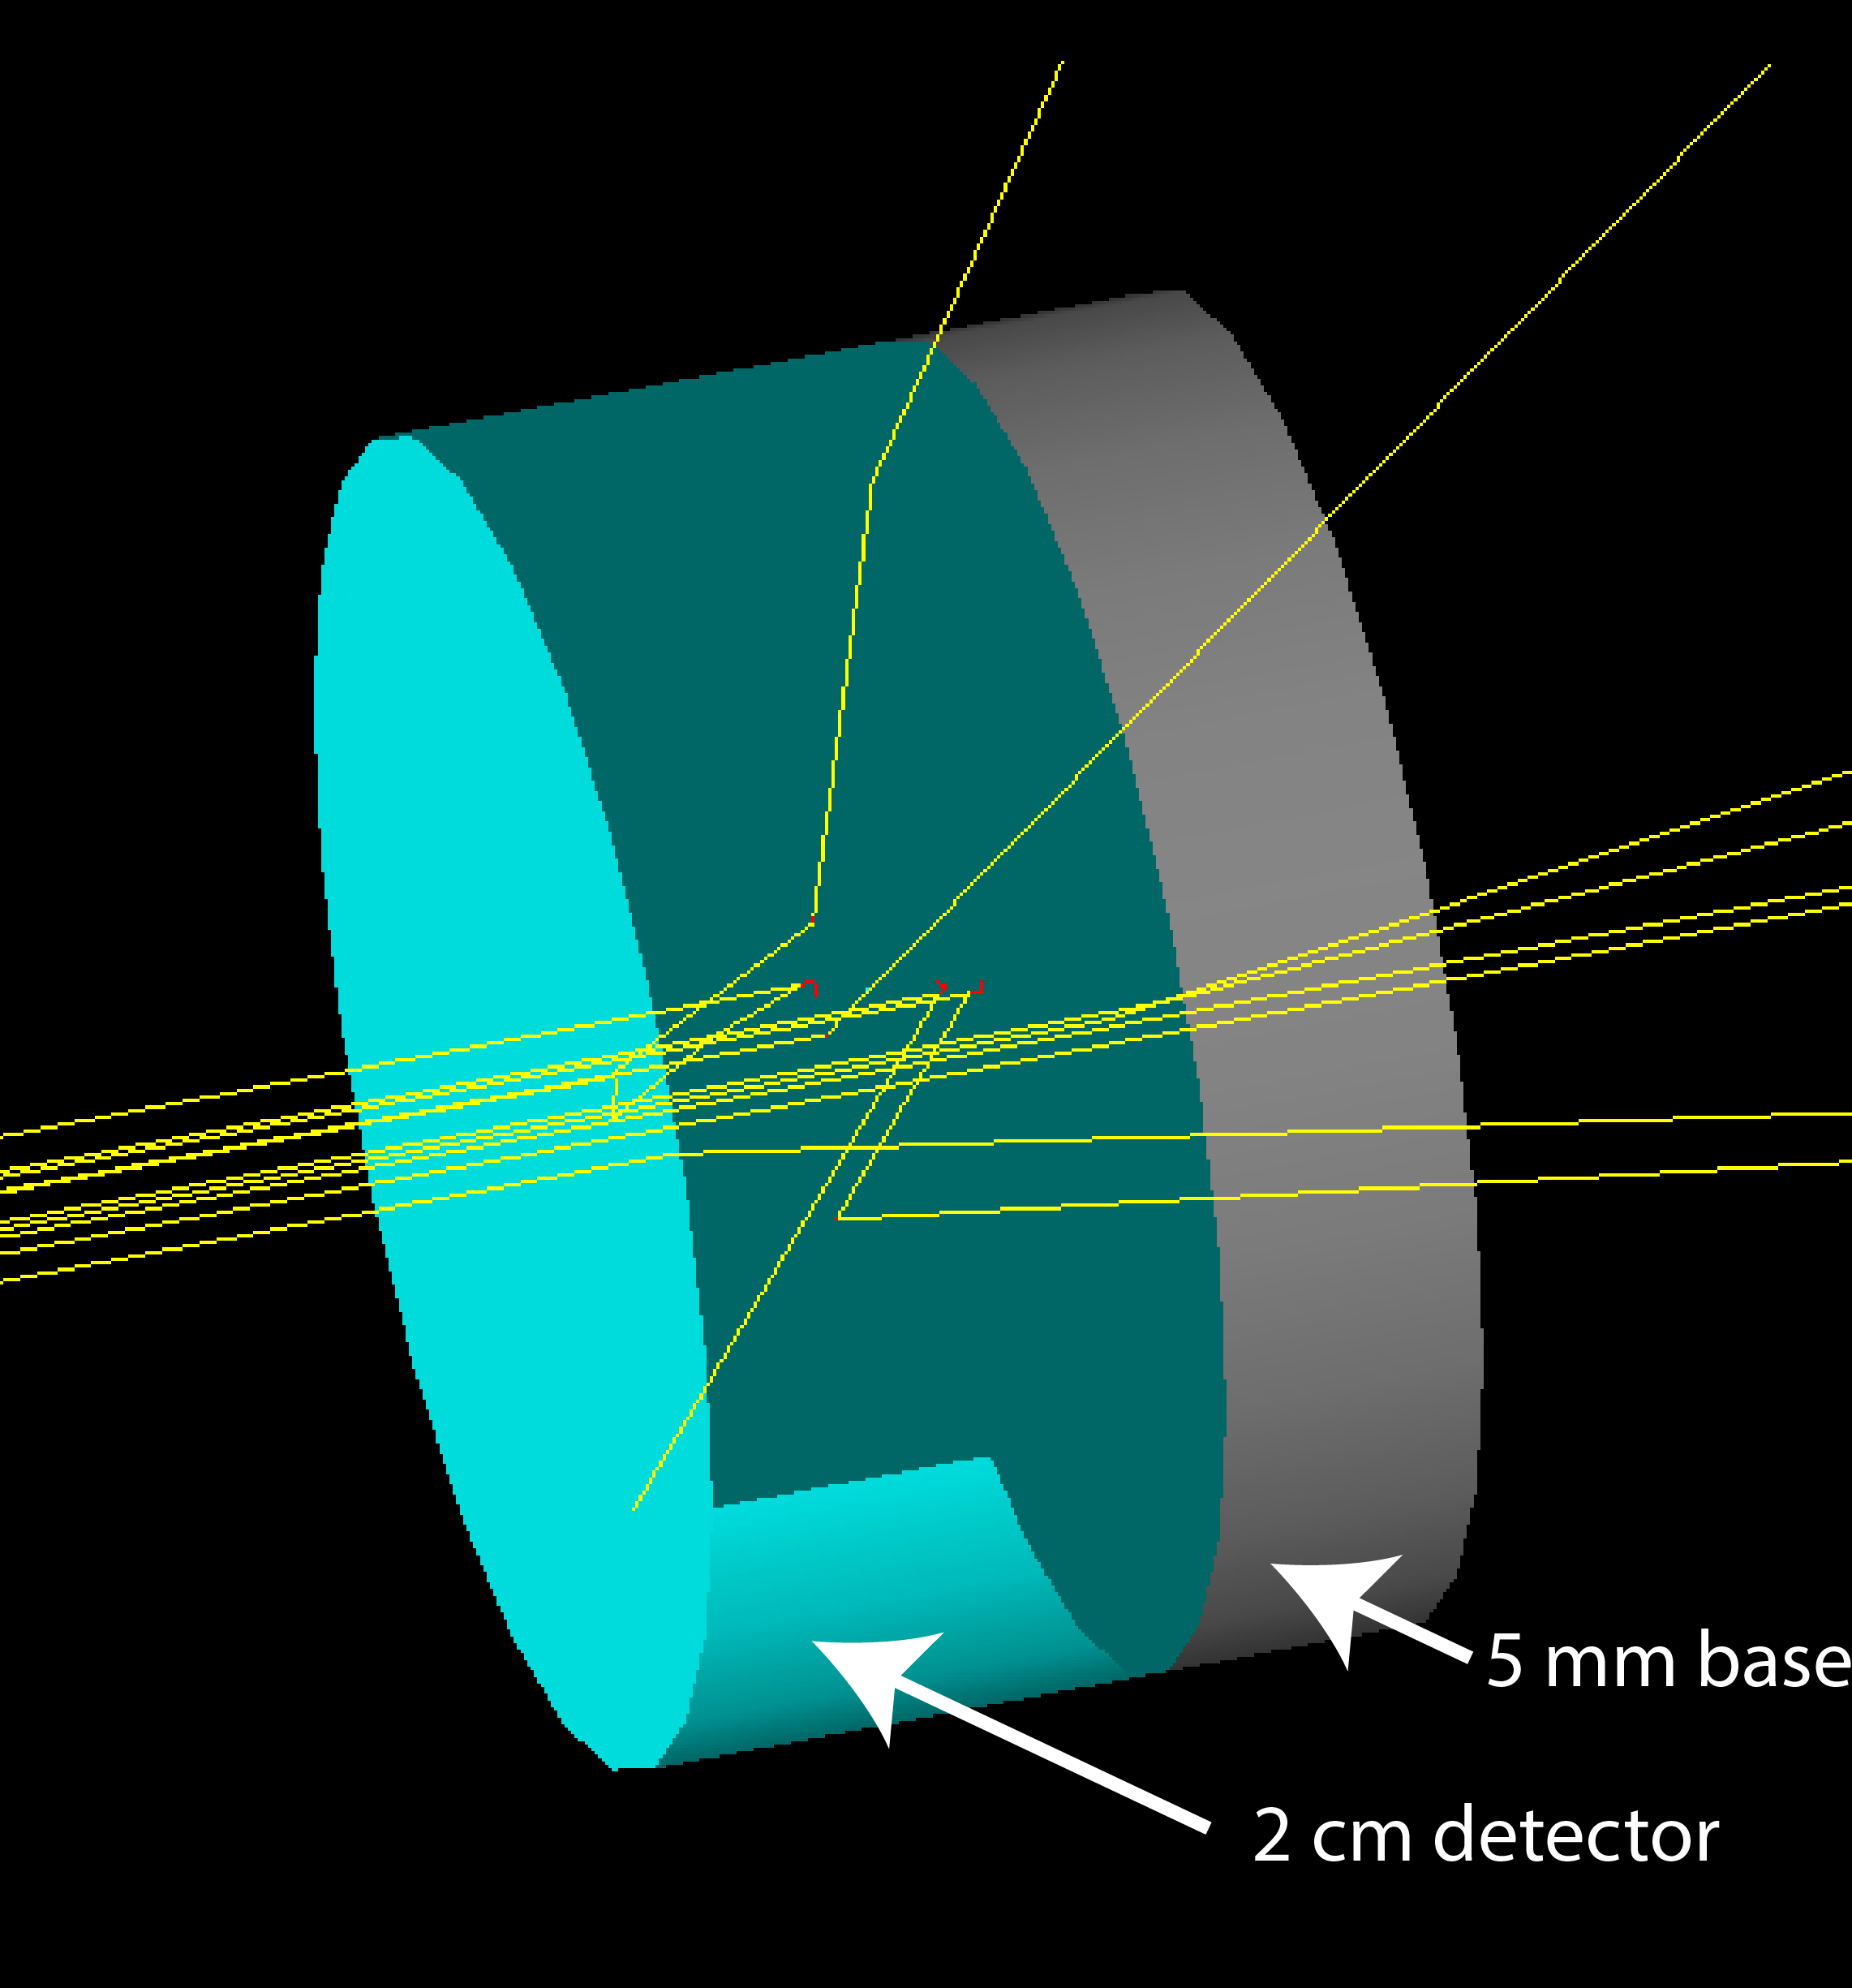
\includegraphics[width=\textwidth]{GEANT4AnnotatedGeo_EnergyDepEvent}
	\caption[GEANT4 Energy Deposition Geometry]{GEANT4 Geometry for the Simulation of Energy Deposition. What is shown are 10 photons from a \iso[60]{Co} source impingement upon a \SI{2}{\cm} thick detector.  The photon tracks are shown in yellow, while the electron tracks are shown in red.}
	\label{fig:EDepSimGeo}
\end{figure}
It is expected that the the Livermore data-driven parameterized electromagnetic physics will be necessary to calculate the ionizing energy deposition, extending the standard electro-magnetic physics down to \SI{1}{\kilo\eV}.
The neutron interactions will be simulated with a hadronic modules, using the \verb+HP+ flavored modules to use the ENDF cross sections to calculate the interaction rates.

\subsubsection{Energy Deposition Validation}
The validation of this GEANT4 simulation was completed by reproducing the single collision energy loss in water as well as comparing  the spectral shapes and averages of simulated and measured spectra.
The reproduction of the single collision energy loss will ensure that the electron physics are implemented correctly, while the simulation of the polymeric film energy deposition allows the user to gain confidence that the correct tracking and binning analysis has been implemented.

The simulation was validated by reproducing the single collision energy loss for water as well as comparing spectra shapes and averages of simulated spectra to the measured spectra.
The single collision energy loss spectra for water that was simulated is shown in \autoref{fig:SingleCollisionELossWater}.
In general there was excellent agreement between the simulated energy spectra and a previously published spectra\cite{turner_comparative_1982}, with the simulated spectra having much better resolution than the reference did not.
It is thought that this is due to the water model in GEANT4 having better cross sections than the previously published spectra.
\begin{figure}
  \centering
  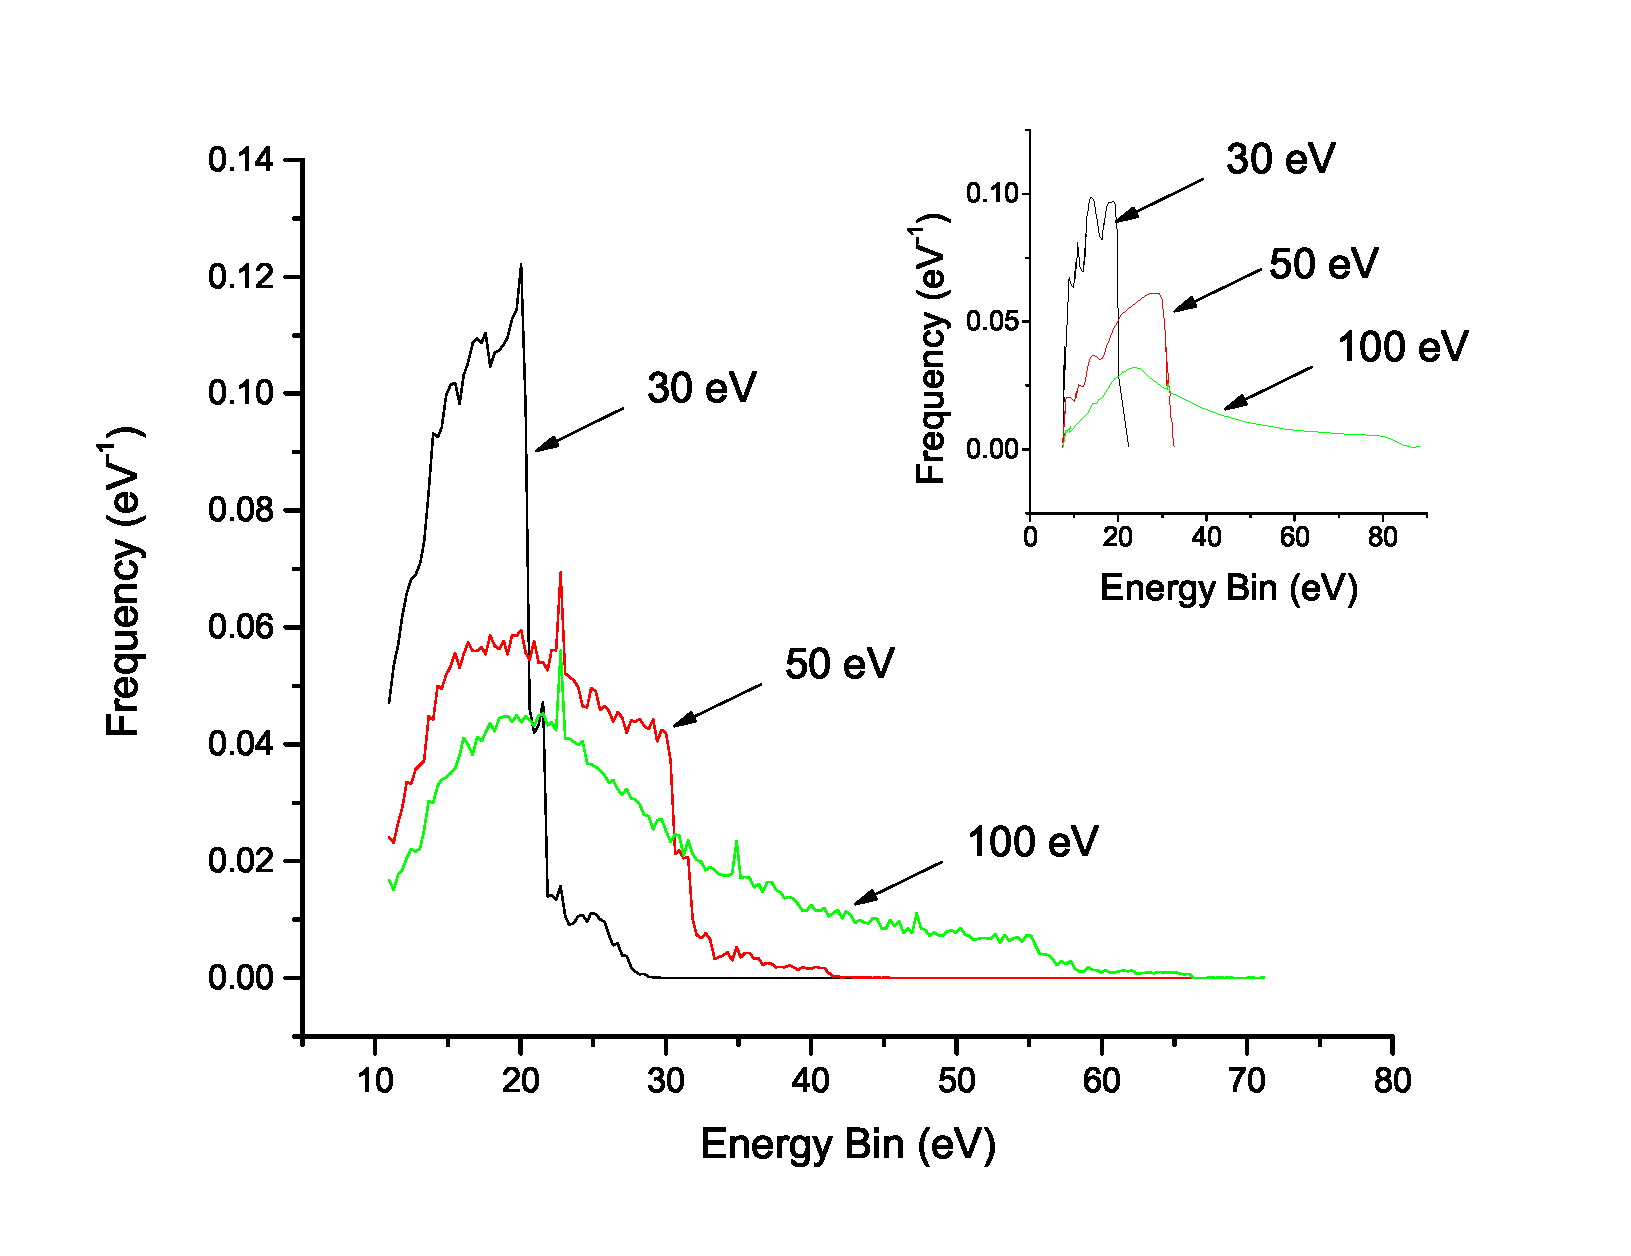
\includegraphics[width=\textwidth]{SingleCollsionEnergyLoss_Turner.eps}
  \caption[Single Collision Energy Loss of Water]{Simualted single collision energy loss of electrons in water. The GEANT simulated ata is shown in the foreground, while the insert contains the data from \cite{turner_comparative_1982}.}
	\label{fig:SingleCollisionELossWater}
\end{figure}

The validity of the GEANT4 simulation is determined by comparing the spectra shapes of measured spectra to simulated energy deposition.
Example gamma simulated spectra are shown in \autoref{fig:G4SimulatedEDep}, where for thin films there is an almost linear increase in the spectra endpoints with film thickness.
The simulated energy deposition per incident photon from a \iso[60]{Co} source and the measured pulse height spectra from the \iso[60]{Co} irradiator per incident photon can be compared by finding a calibration between them, in this case the Compton edge of a thick sample.
The measured Compton edge of a \SI{1}{\mm} film can then be correlated with the simulated energy, as shown in \autoref{fig:spectraComparisonGamma}.
The energy of this feature on the measured spectra was then compared to the energy on the simulated spectra, with all of the values being within 10\%.
\begin{figure}
	\centering
    	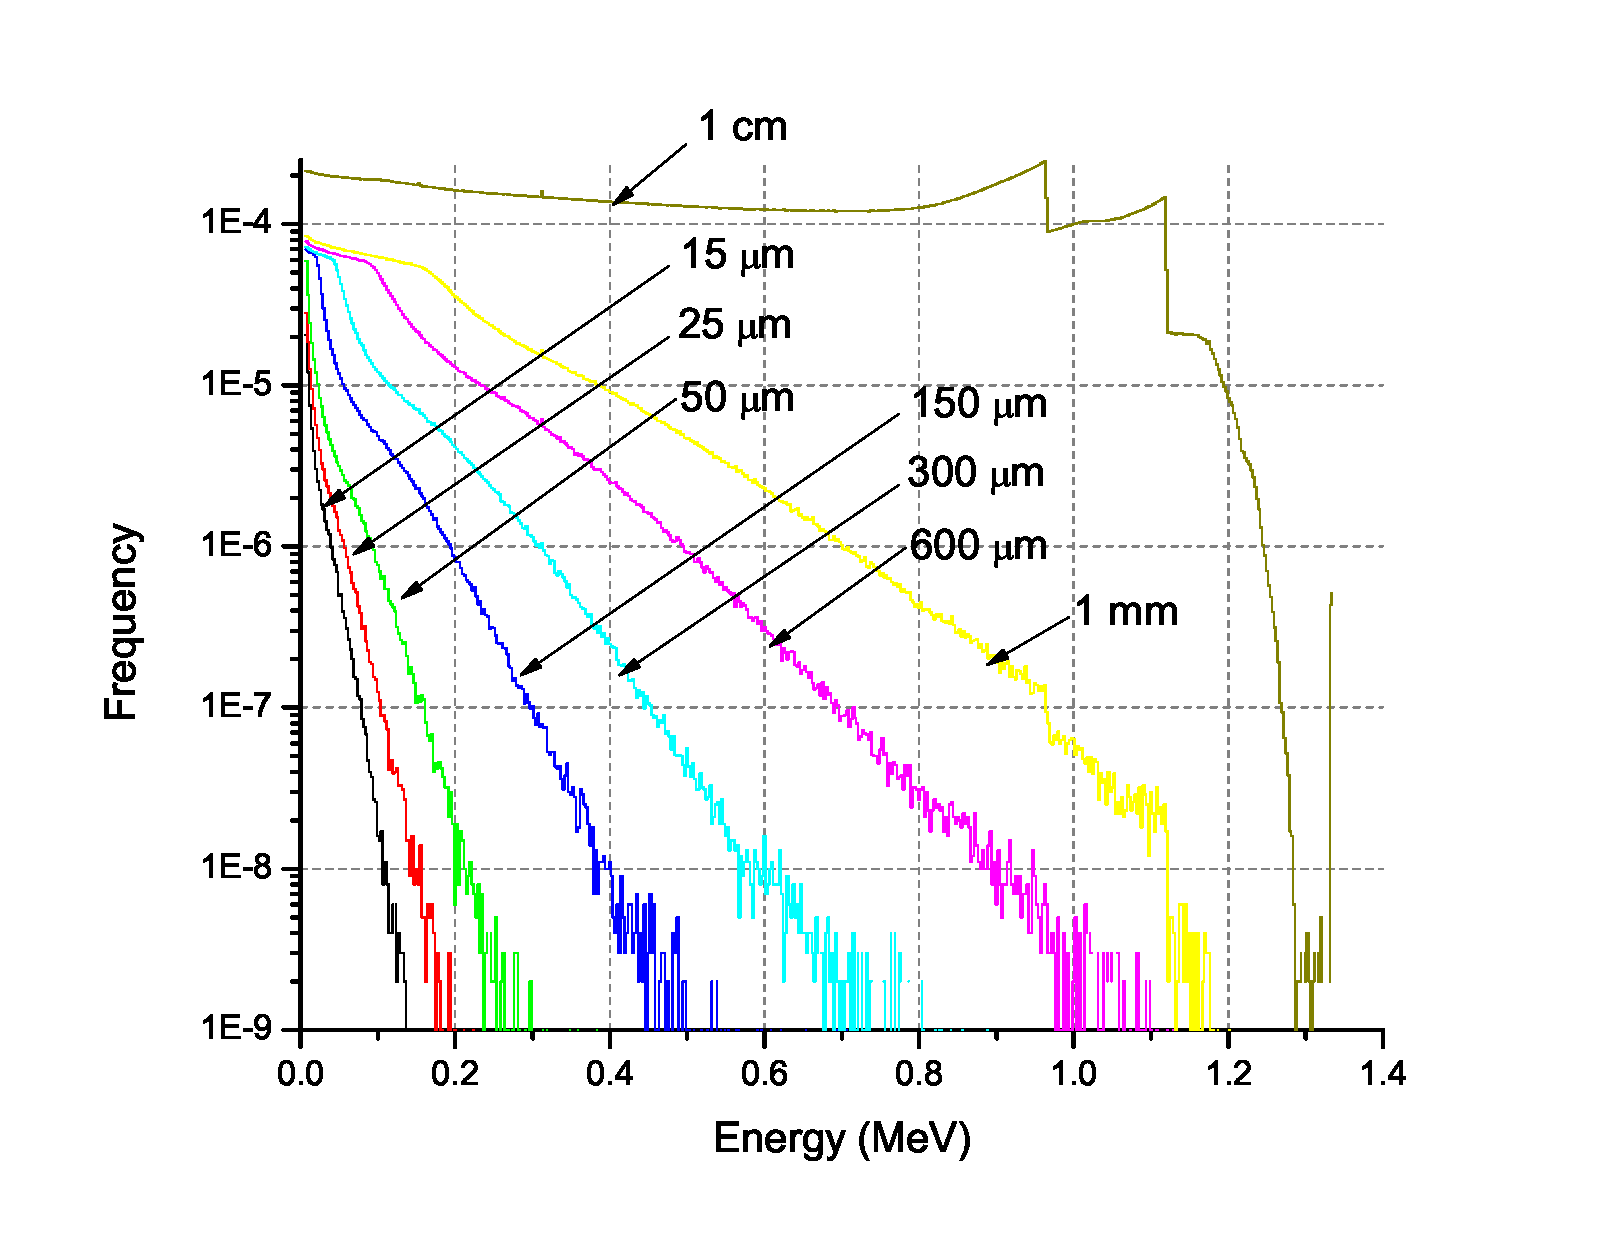
\includegraphics[width=\textwidth]{PS_EDepSim_Co60}
	\caption[GEANT4 Simulated Gamma Spectra in PS]{GEANT4 simulated energy deposition from incident the \SI{1.17}{\MeV} and \SI{1.33}{\MeV} photons of \iso[60]{Co} in polystyrene films loaded with 10\% \iso[6]{LiF} of different thickness. The Compton edge of the two photons is clearly visiable for the \SI{1}{\cm} film, while the other films show an almost linear increase in energy deposited with thickness.}
	\label{fig:G4SimulatedEDep}
\end{figure}
\begin{figure}
	\centering
   	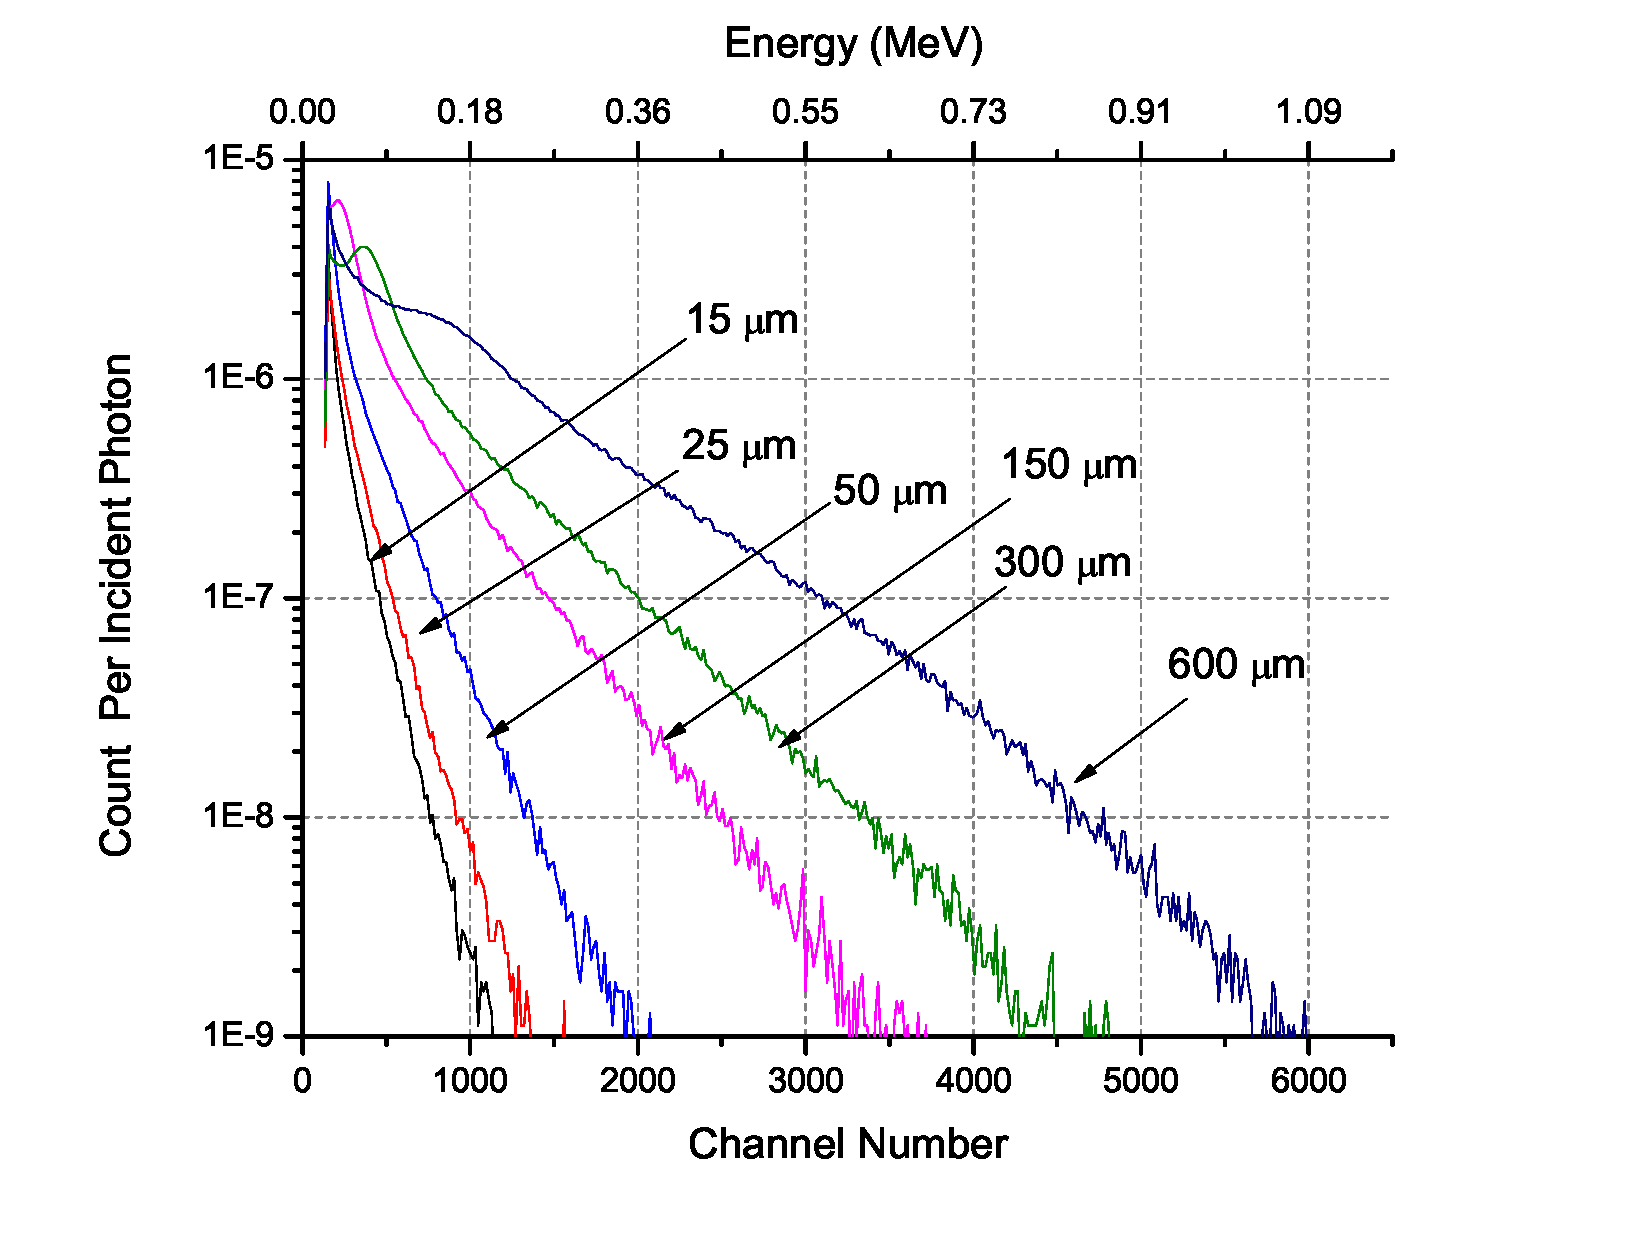
\includegraphics[width=\textwidth]{PS_GammaCR-Binned-FluxNorm_20LiF_5PPO}
	\caption{Comparison of the energy deposition and binned pulse height spectra for 10\% loaded polystyrene from a \iso[60]{Co} source. The simulated and measured spectra have the same shape, indicating agreement. The fabricated films greater than \SI{600}{\um} were of poor optical quality and therefore their results are not shown. }
	\label{fig:spectraComparisonGamma}
\end{figure}

A direct comparison between the simulated average energy deposition and pulse height are shown in \autoref{fig:EDepLightYieldNeutron} and \autoref{fig:EDepLightYieldGamma}. 
The average energy deposition is shown on the left axis and the average light yield (pulse height) on the right axis.
The largest amount of energy that can be deposited in the neutron interaction is \SI{4.78}{\MeV}, which is approached after \SI{200}{\um} in both the measurement and simulations.
This asymptotic behavior is not observed for the gamma spectra.
\begin{figure}
	\centering
    	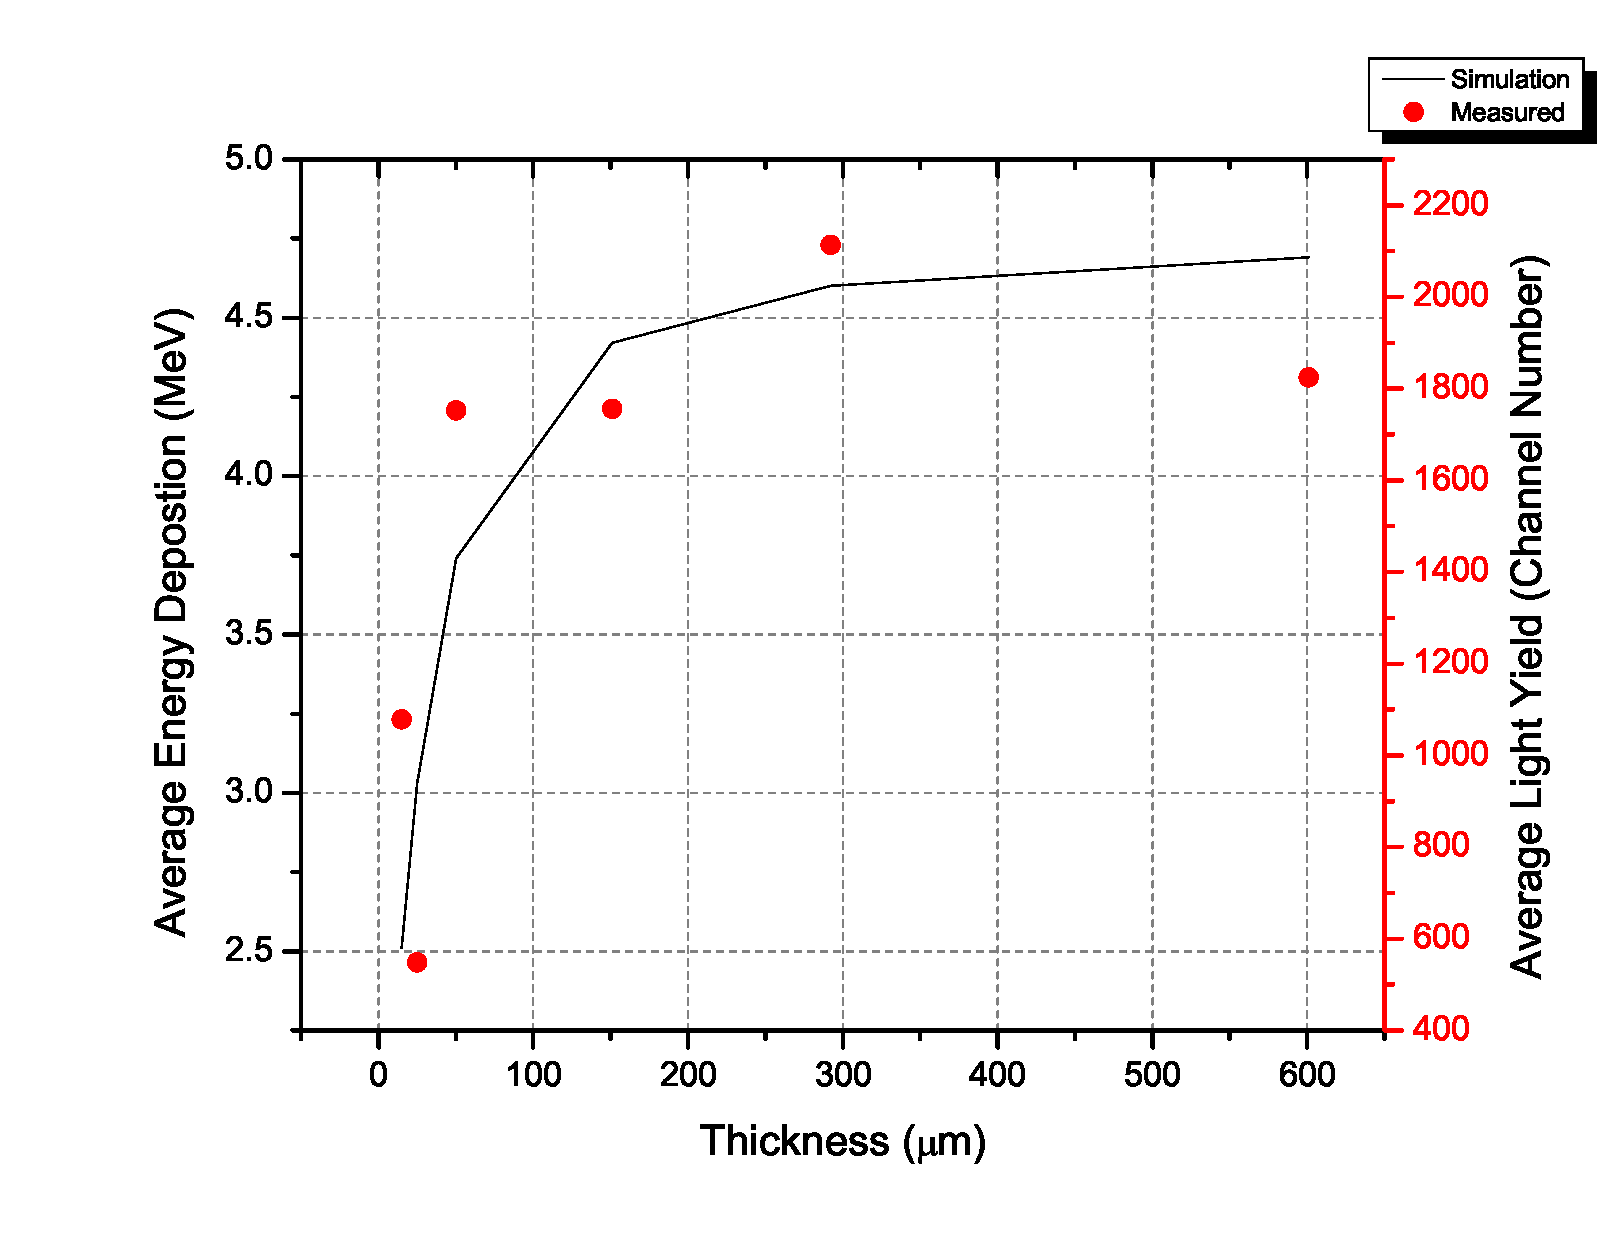
\includegraphics[width=\textwidth]{G4EDep_LightYield_Neutron}
	\caption[Average Light Yield and Energy Deposition for neutron interactions in PS]{Average energy deposition and measured light yield for neutron interactions in 10 \% loaded polystyrene. The solid lines are calculated values and the red dots are measurements. The incident particle for the simulation is a neutron of energy \SI{0.025}{\eV}, while the measured is the response of thermal neutron spectrum measured from the Cf-252 irradiator. The reaction products depositing the energy are an alpha and a triton.}
	\label{fig:EDepLightYieldNeutron}
\end{figure}
\begin{figure}
	\centering
    	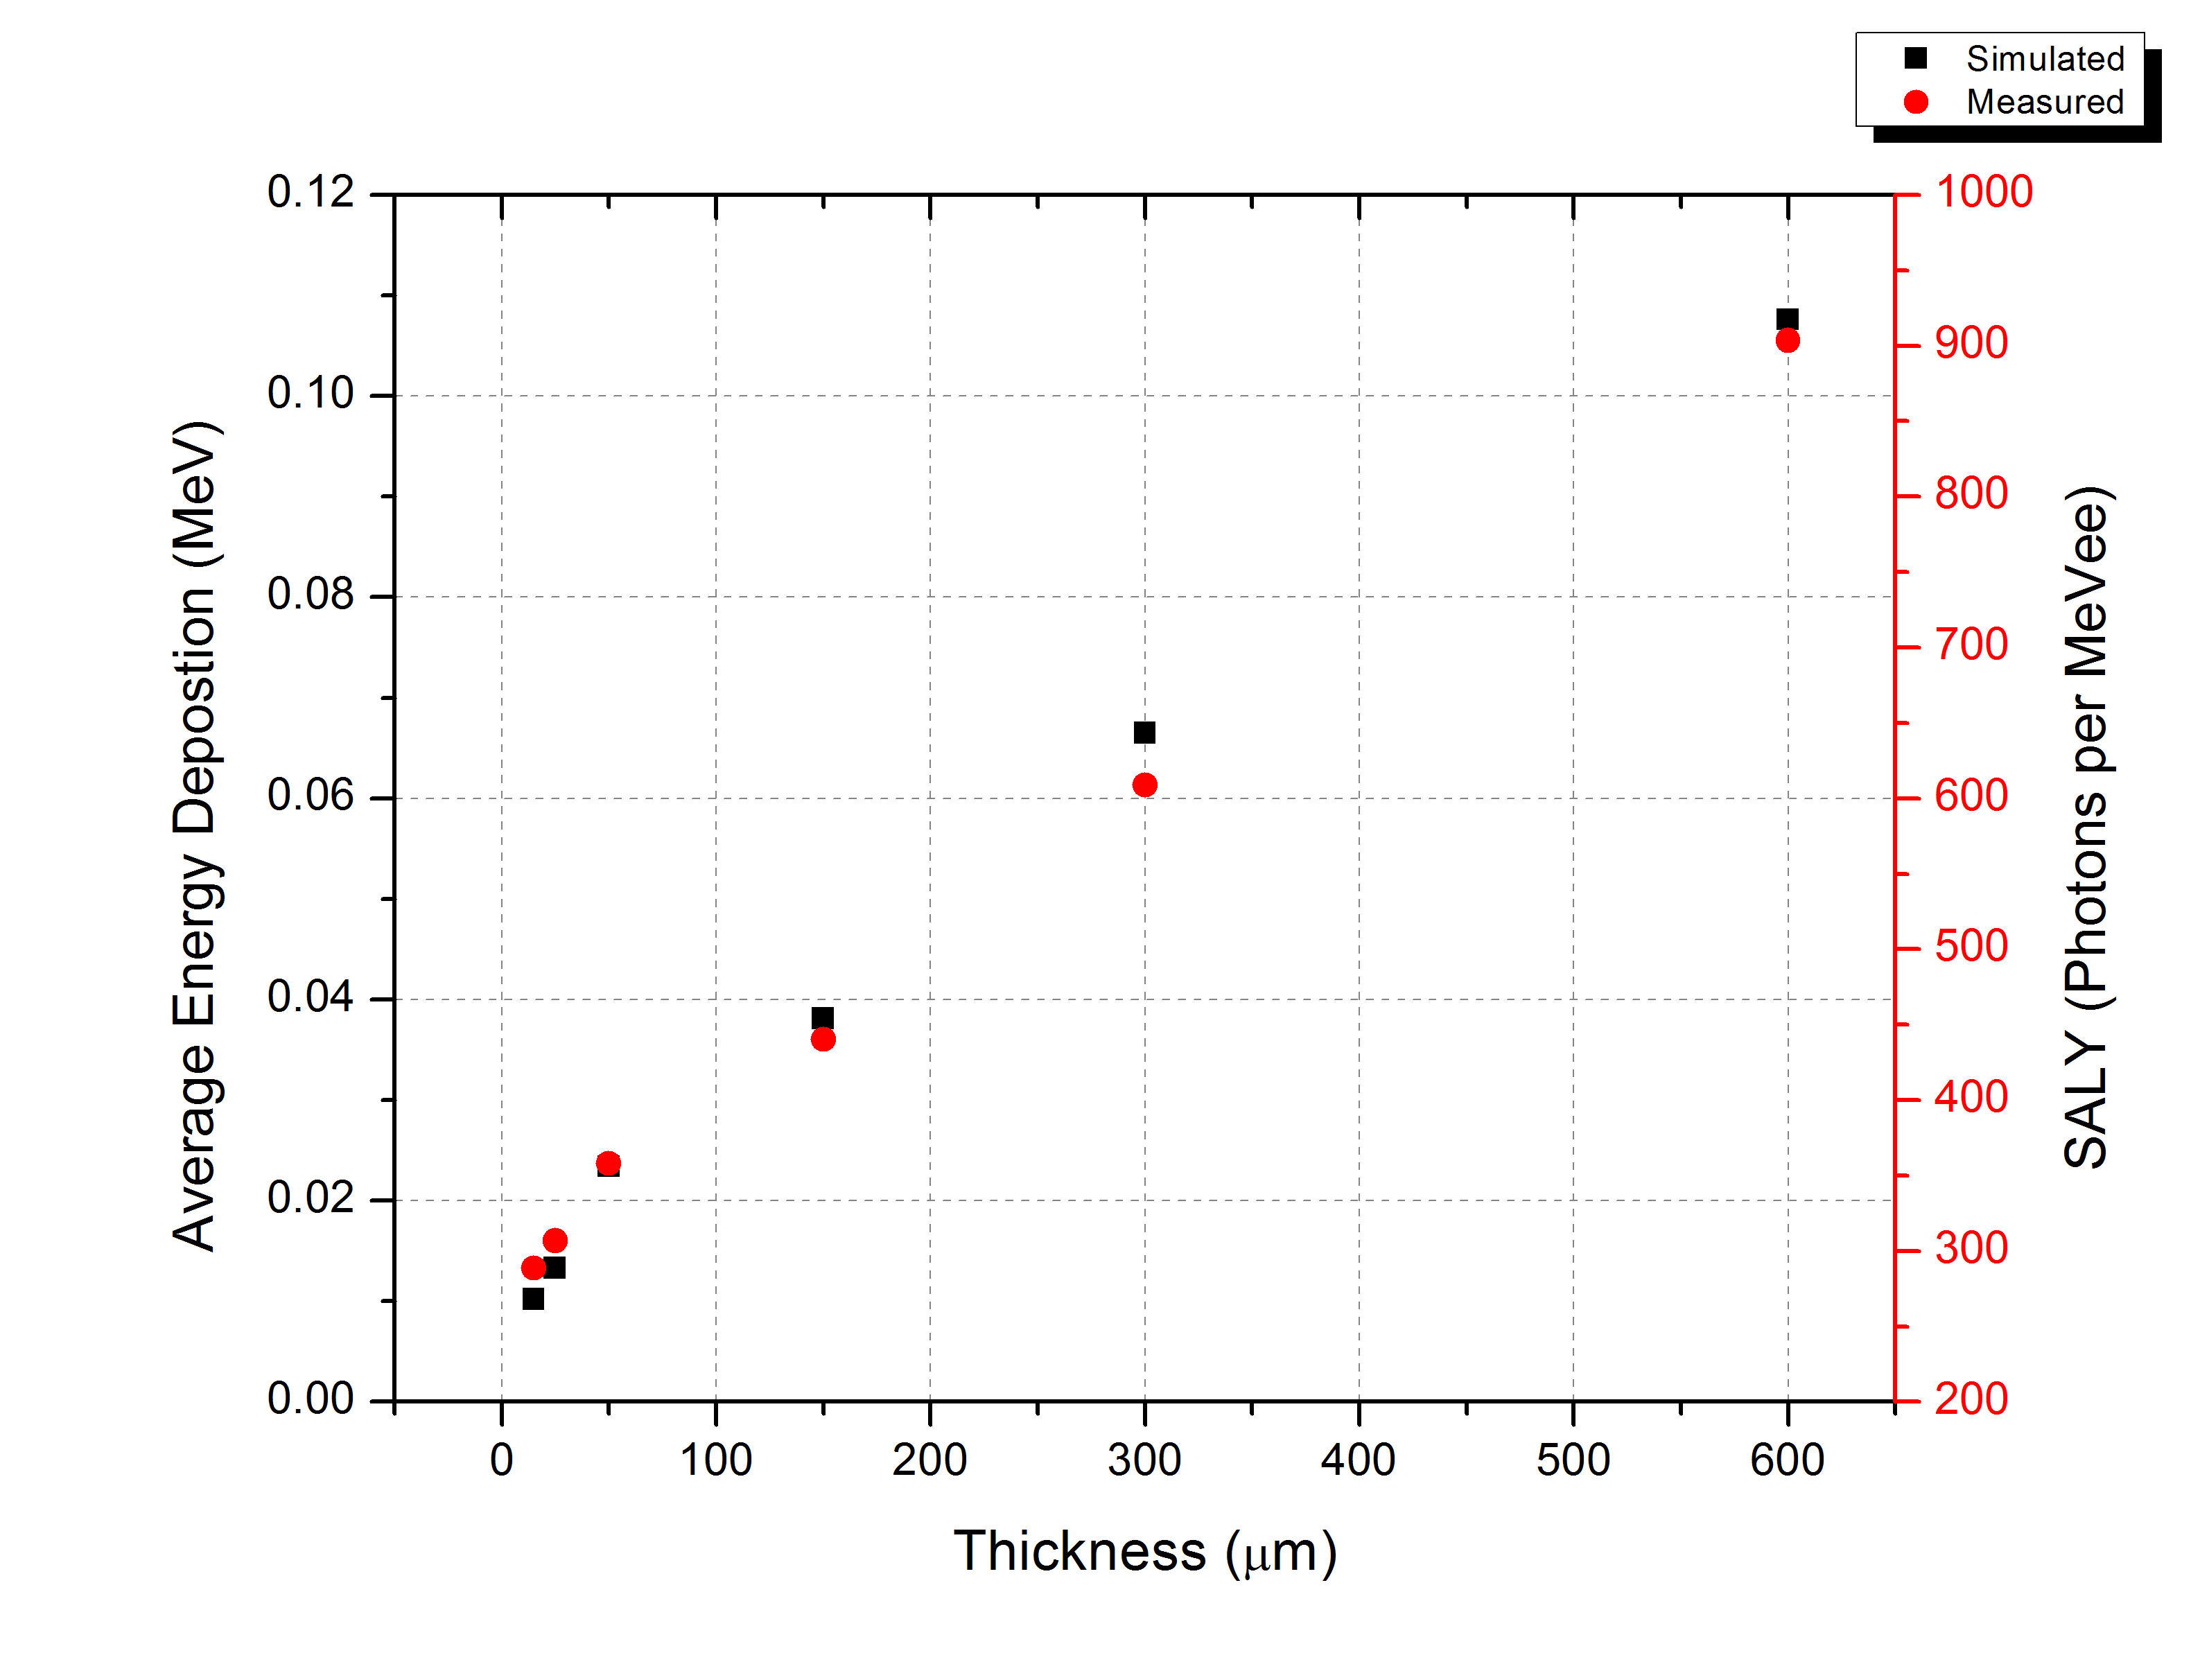
\includegraphics[width=\textwidth]{G4EDep_LightYield_Co60}
	\caption[Average Light Yield and Energy Deposition for Gamma interactions in PS]{Average energy deposition and measured light yield for \iso[60]{Co} interactions in 10 \% loaded polystyrene. The solid lines are calculated values and the red dots are measurements. The maximum amount of energy that could be deposited by a \iso[60]{Co} photon is \SI{1.33}{\MeV}.}
	\label{fig:EDepLightYieldGamma}
\end{figure}

\subsection{Optical Photon Simulations}
\label{sec:OpticalPhotonSims}
Photons are considered to be optical photons in the GEANT4 model when the wavelength of the photon is much greater than atomic spacing to allow for their wave-like nature.
Optical photons were simulated in GEANT4 by creating an optical material property for each of the optical materials.
In general this involves setting the scintillation yield of the material, the resolution of the material, the optical photon absorbance of the film, the decay time, and the Birks parameter of the material to simulate the light quenching of the material.
Scattering at the boundary between two surfaces can be  handled by the UNIFIED model for Optical Surfaces, by the use of look up tables based on the measured data values \cite{5485130}, or simply based on the index on Snell's law.
For this work a look up table model was employed.


\subsection{Optical Photon Yield}
\label{sec:OpticalPhotonValidation}
The GEANT4 optical photon model was verified by measuring a detector and then simulating a similar detector in the GEANT4 toolkit. 
The comparison of the simulated entire  detection mechanisms (including the energy deposition, scintillation, and optical photon collection) to the a measured value provides confidence in the entire model; however, it should be noted that a validation of this type could allow for individual errors to miraculously cancel each other out.
Two cases where considered for the validation: 1) a sample mounted onto a PMT and 2) fabricated layered detectors that where  \SI{10}{cm} by \SI{15}{cm} by \SI{6}{cm} .
The single sample mounted on the PMT was used to establish the Birks constant for the material and the light yield (more details can be found in \autoref{sec:G4OpticalPhysicsAppendix}), and the fabricated layered detectors measurements were used to provide confidence of the ability to simulate a large scale detector system.

A single sample mounted on a PMT provides a simple geometry to validate the parameters used in the light transport simulations. 
The geometry consist of a sample mounted with a thin layer of optical grease to the PMT, and the entire assembly is wrapped with teflon grease, as shown in \autoref{fig:SingleDetectorLightValGeo}.
This mimics the measurement of a sample mounted on a PMT, expect for the efficiency of the photocathode is not considered.
The simulated neutron and gamma optical photon spectra for GS20 and polystyrene based film are shown in \autoref{fig:GS20LightVal} and \autoref{fig:PSLightVal}.
\begin{figure}
	\centering
	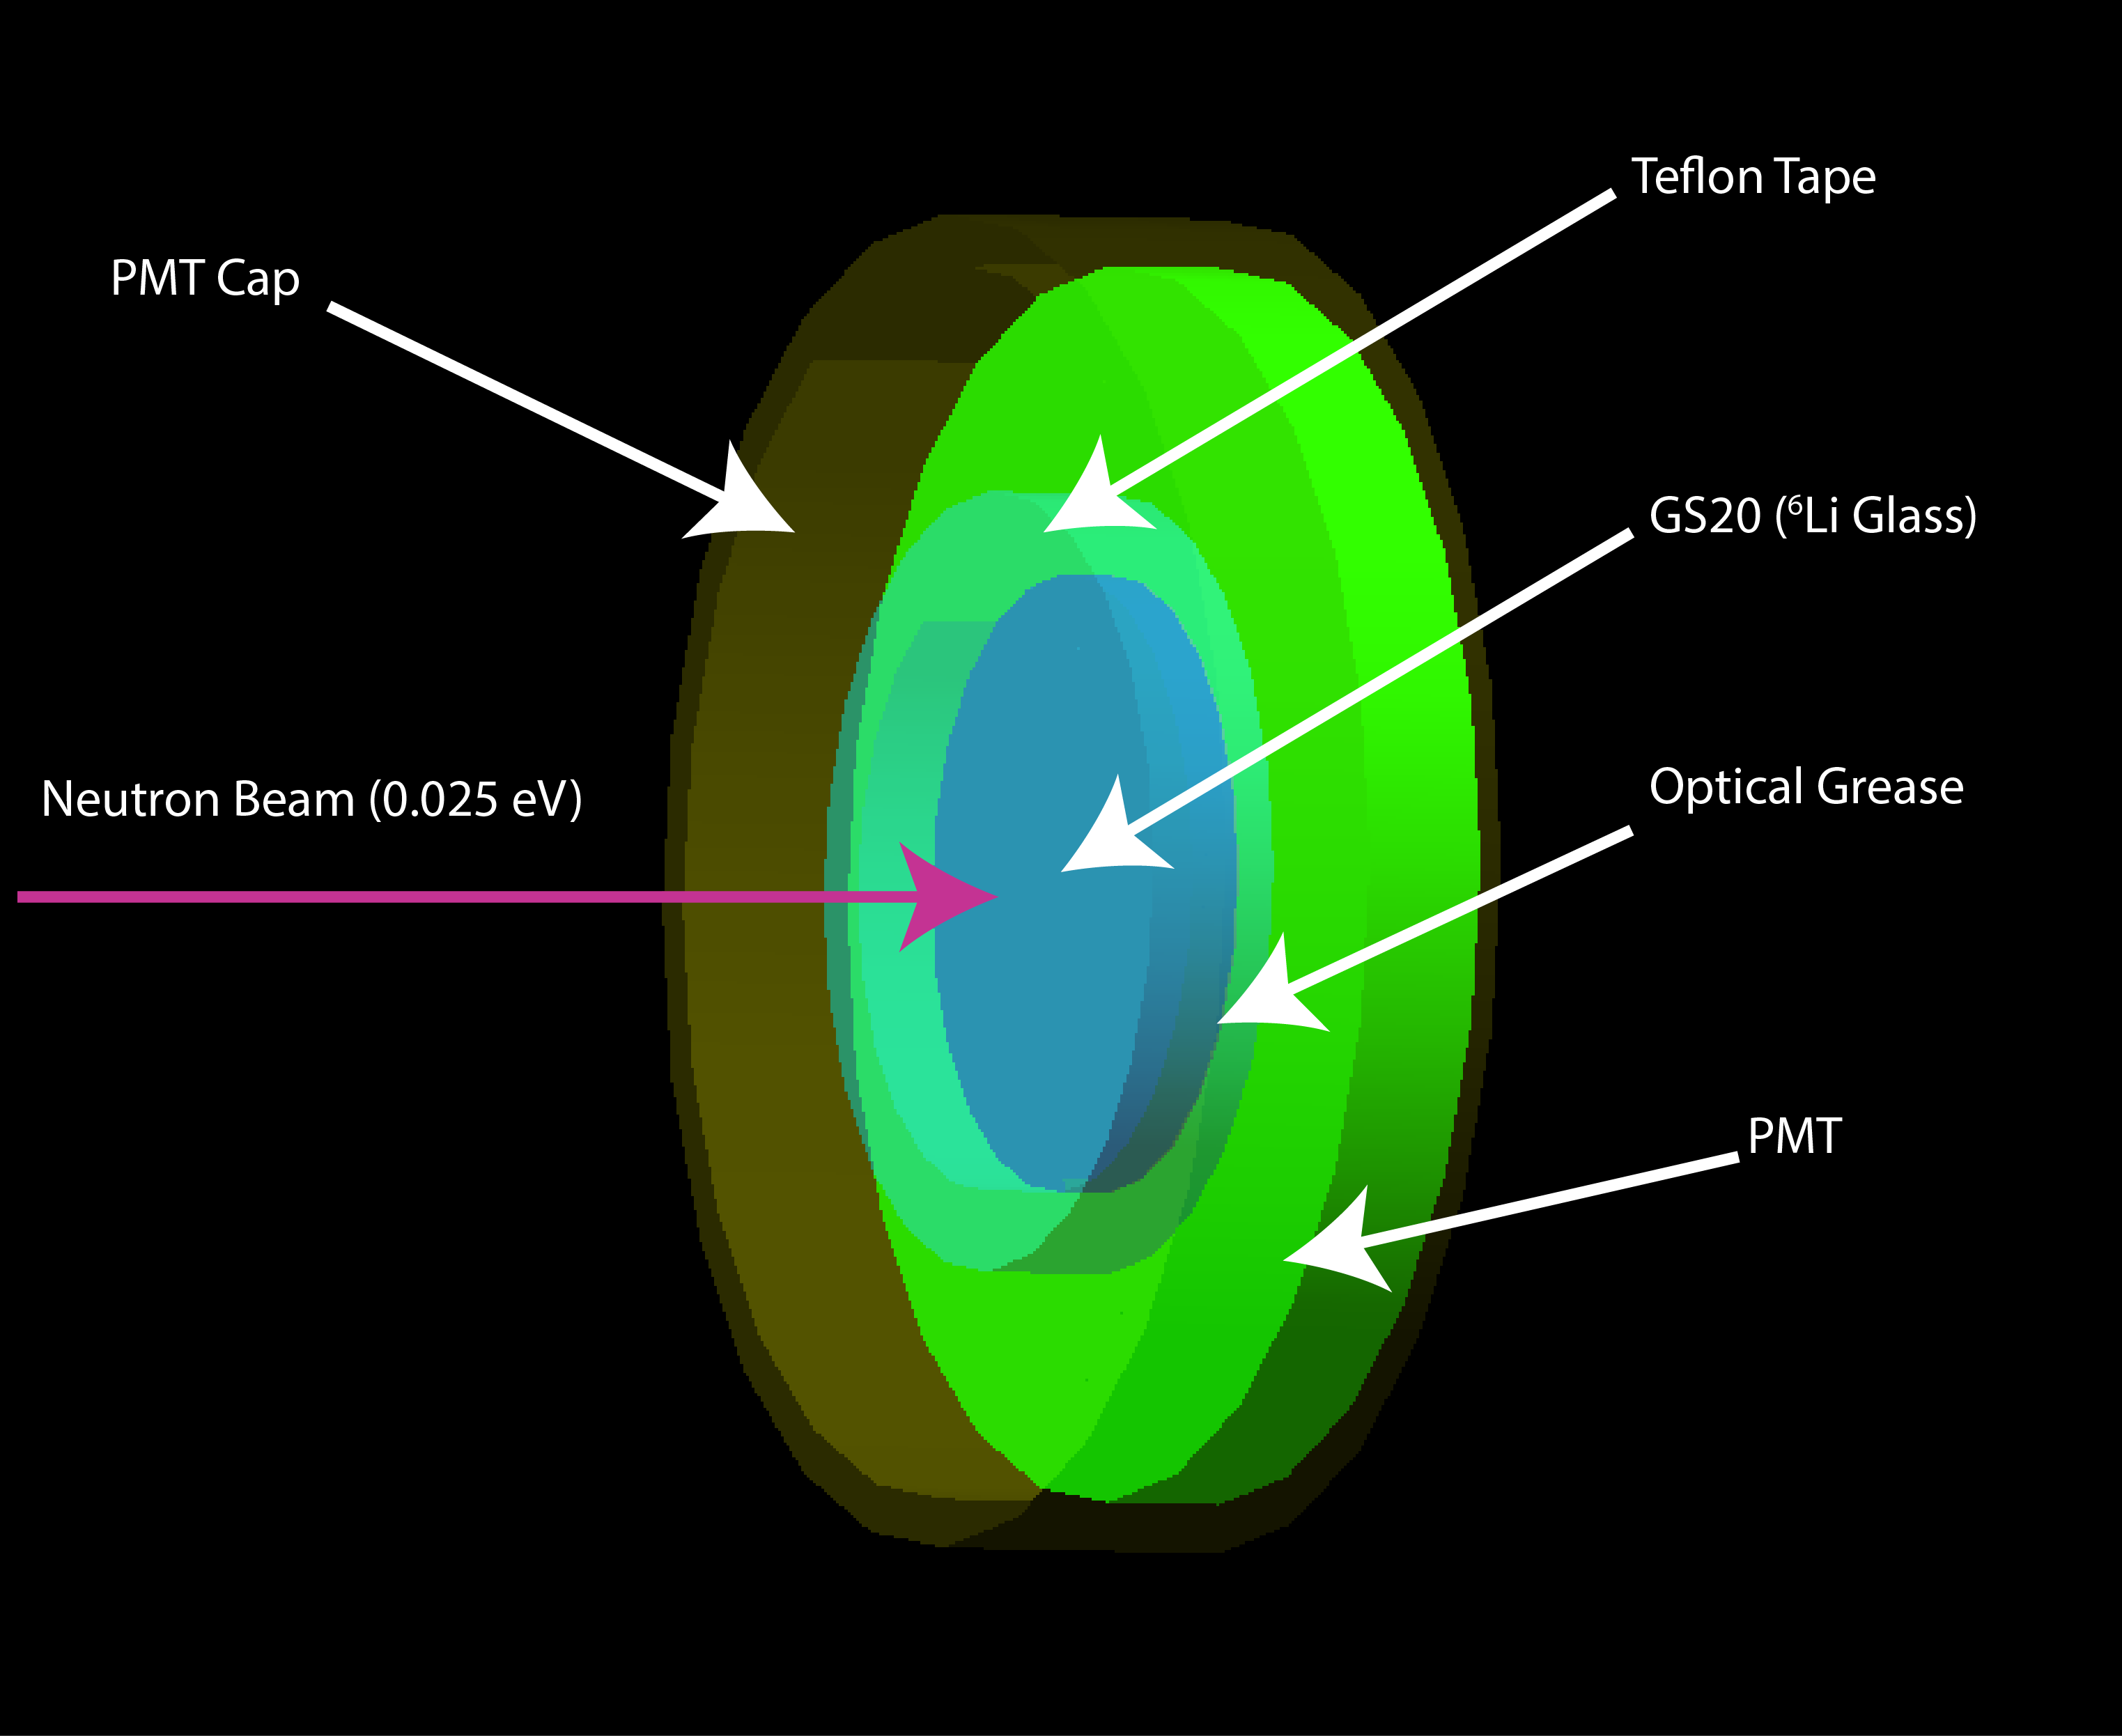
\includegraphics[width=\textwidth]{GEANT4AnnotatedGeo_GS20SimGeo}
	\caption[Simulated Detector Geoemtry for Single Detectors]{Simulated detector geometries for the single detector light collection validation. The two detector materials used in the study are GS20 and ten precent \iso[6]{LiF} polystyrene.}
	\label{fig:SingleDetectorLightValGeo}
\end{figure}
\begin{figure}
	\centering
	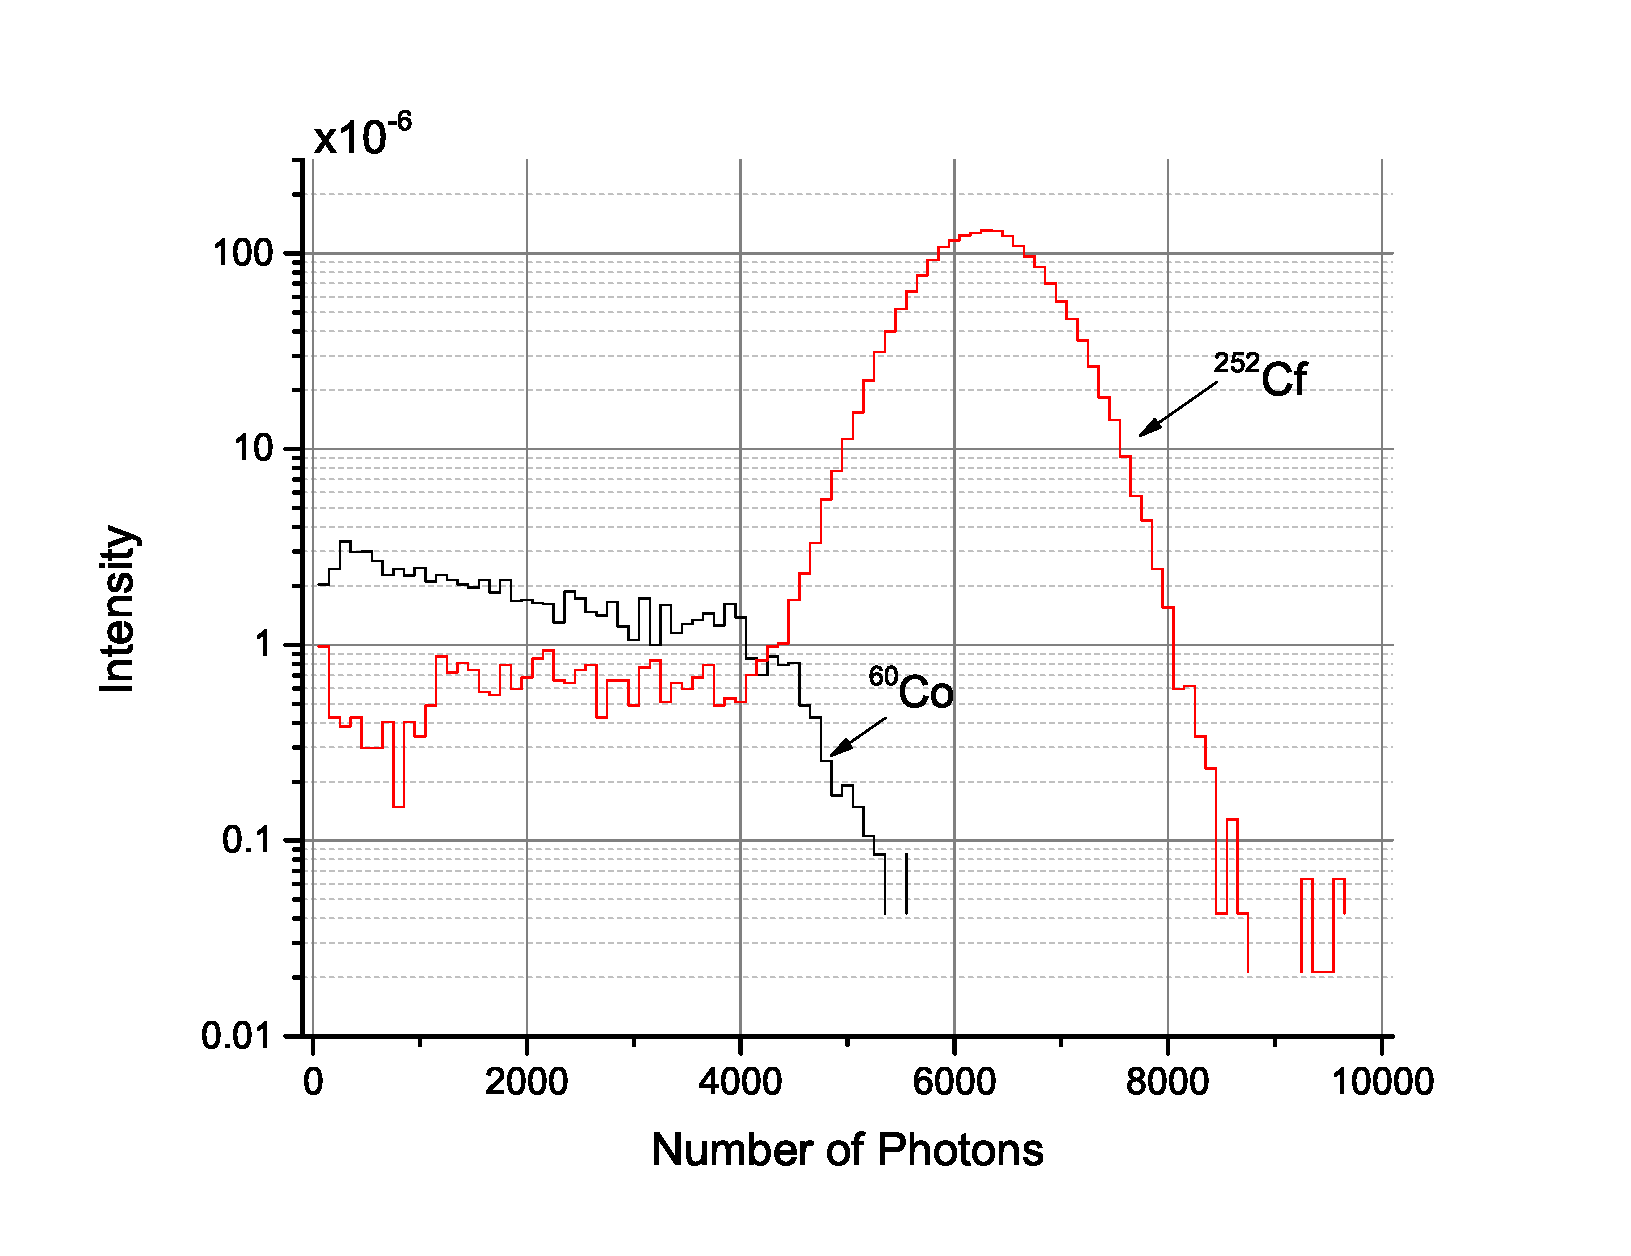
\includegraphics[width=\textwidth]{LightValidation_GS20.eps}
	\caption{Simulated Gamma and Neutron Optical Photon Distribution in GS20. \LightYieldEDepSimGeo}
	\label{fig:GS20LightVal}
\end{figure}
\begin{figure}
	\centering
	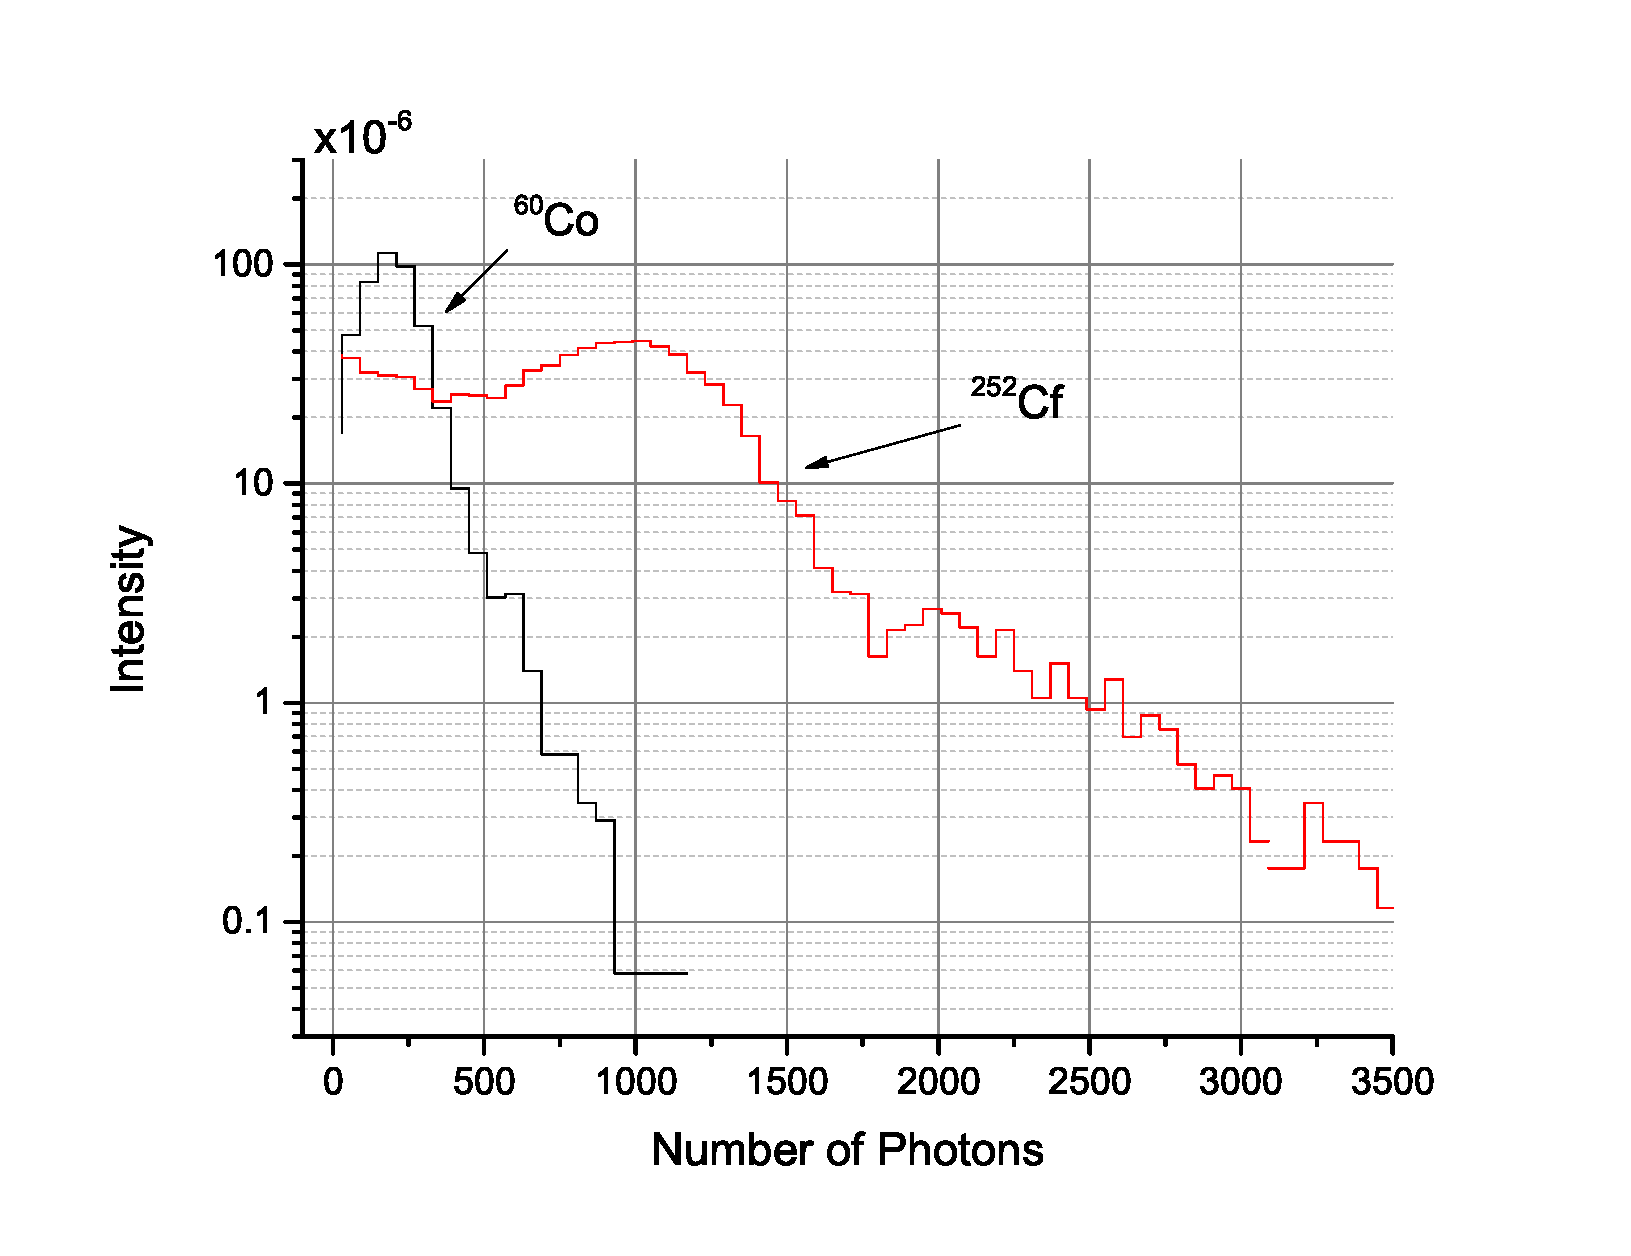
\includegraphics[width=\textwidth]{LightValidation_PS.eps}
	\caption{Simulated Gamma and Neutron Optical Photon Distribution for a polystyrene film. \LightYieldEDepSimGeo}
	\label{fig:PSLightVal}
\end{figure}

The large scale transport of optical photons with the different boundary processes simulation was validated by measuring four assemblies of \SI{10.16}{\cm} by \SI{15.24}{\cm} scintillators with an attached fishtail light guide.
Two of the samples where a 10\% loaded \iso[6]{LiF} polystyrene cast to \SI{50}{\um} and \SI{100}{\um}, while the other samples were a \SI{100}{\um} \iso[6]{LiF} loaded ZnS:Ag (purchased from Eljen, EJ-426) and a recast carborane sample from South Carolina State University.
The PMMA slabs and light guide were also purchased from Eljen Technologies.
The slabs and scintillators were mounted together with optical grease, as shown in \autoref{fig:4by6LightGuide} and \autoref{fig:4by6OpticalMounting}.
\begin{figure}
	\centering
	\includegraphics[width=\textwidth]{MeasLayeredDetector_MountingLayers}
	\caption[4" by 6" Layered Detector Light Guide and Detector Assembly]{Image of the light guide and the layered PMMA slices between cast \iso[6]{LiF} loaded polystyrene detectors.}
	\label{fig:4by6LightGuide}
\end{figure}
\begin{figure}
	\centering
	\includegraphics[width=\textwidth]{MeasLayeredDetector_EJ426Mounting}
	\caption[4" by 6" Layered Detector Optical Mounting]{Image of the optical mounting of the detector slabs to the PMMA. The detector material shown in this sample is EJ-426 (LiF loaded ZnS:Ag) and is opaque.  In the case of the EJ-426 optical grease was only applied to the back face of the detector material per the manufactuers instructrions.}
	\label{fig:4by6OpticalMounting}
\end{figure}

The agreement between the simulated number of optical photons and the measured number of optical photons detected is shown in \autoref{tab:4by6SlabOpVal}, with the measured collected spectra shown in \autoref{fig:4by6MeasSpectra}.
The number of optical photons measured was calibrated by measuring the sample of pure material attached directly to the PMT, and simulating the efficiency of collecting the photons in that geometry.
There are several factors effecting the agreement between the simulation and measurement.
The optical coupling of the simulation was assumed to be perfect without air bubbles, which is not consistent with reality.
The opacity of the films were estimated from their absorbance profiles, which depends on how the sample was mounted in the measurement.
Finally, and probably contributing the largest to the discrepancies, no attempt was made to fine tune the material parameters for the optical grease and teflon than that which was available as an example in the GEANT4 toolkit.
\begin{table}
	\caption[Agreeement between Simulated and Measured Photon Collection in 4" by 6" Slabs]{Agreement between the simulated light collection in the 4" by 6" detector assembiles and the measurements.}
	\label{tab:4by6SlabOpVal}
	\begin{tabular}{m{4cm} m{3cm} m{3cm}}
	\toprule
	Sample & Measured Photons Collected & Simulated Photons Collected \\
	\midrule
	EJ-426 & 1, 500 & 2,100 \\
	PS LiF, \SI{50}{\um} & 220 & 260 \\
	PS LiF, \SI{100}{\um} & 100 & 130 \\
	\bottomrule
	\end{tabular}
\end{table}
\begin{figure}
	\centering
	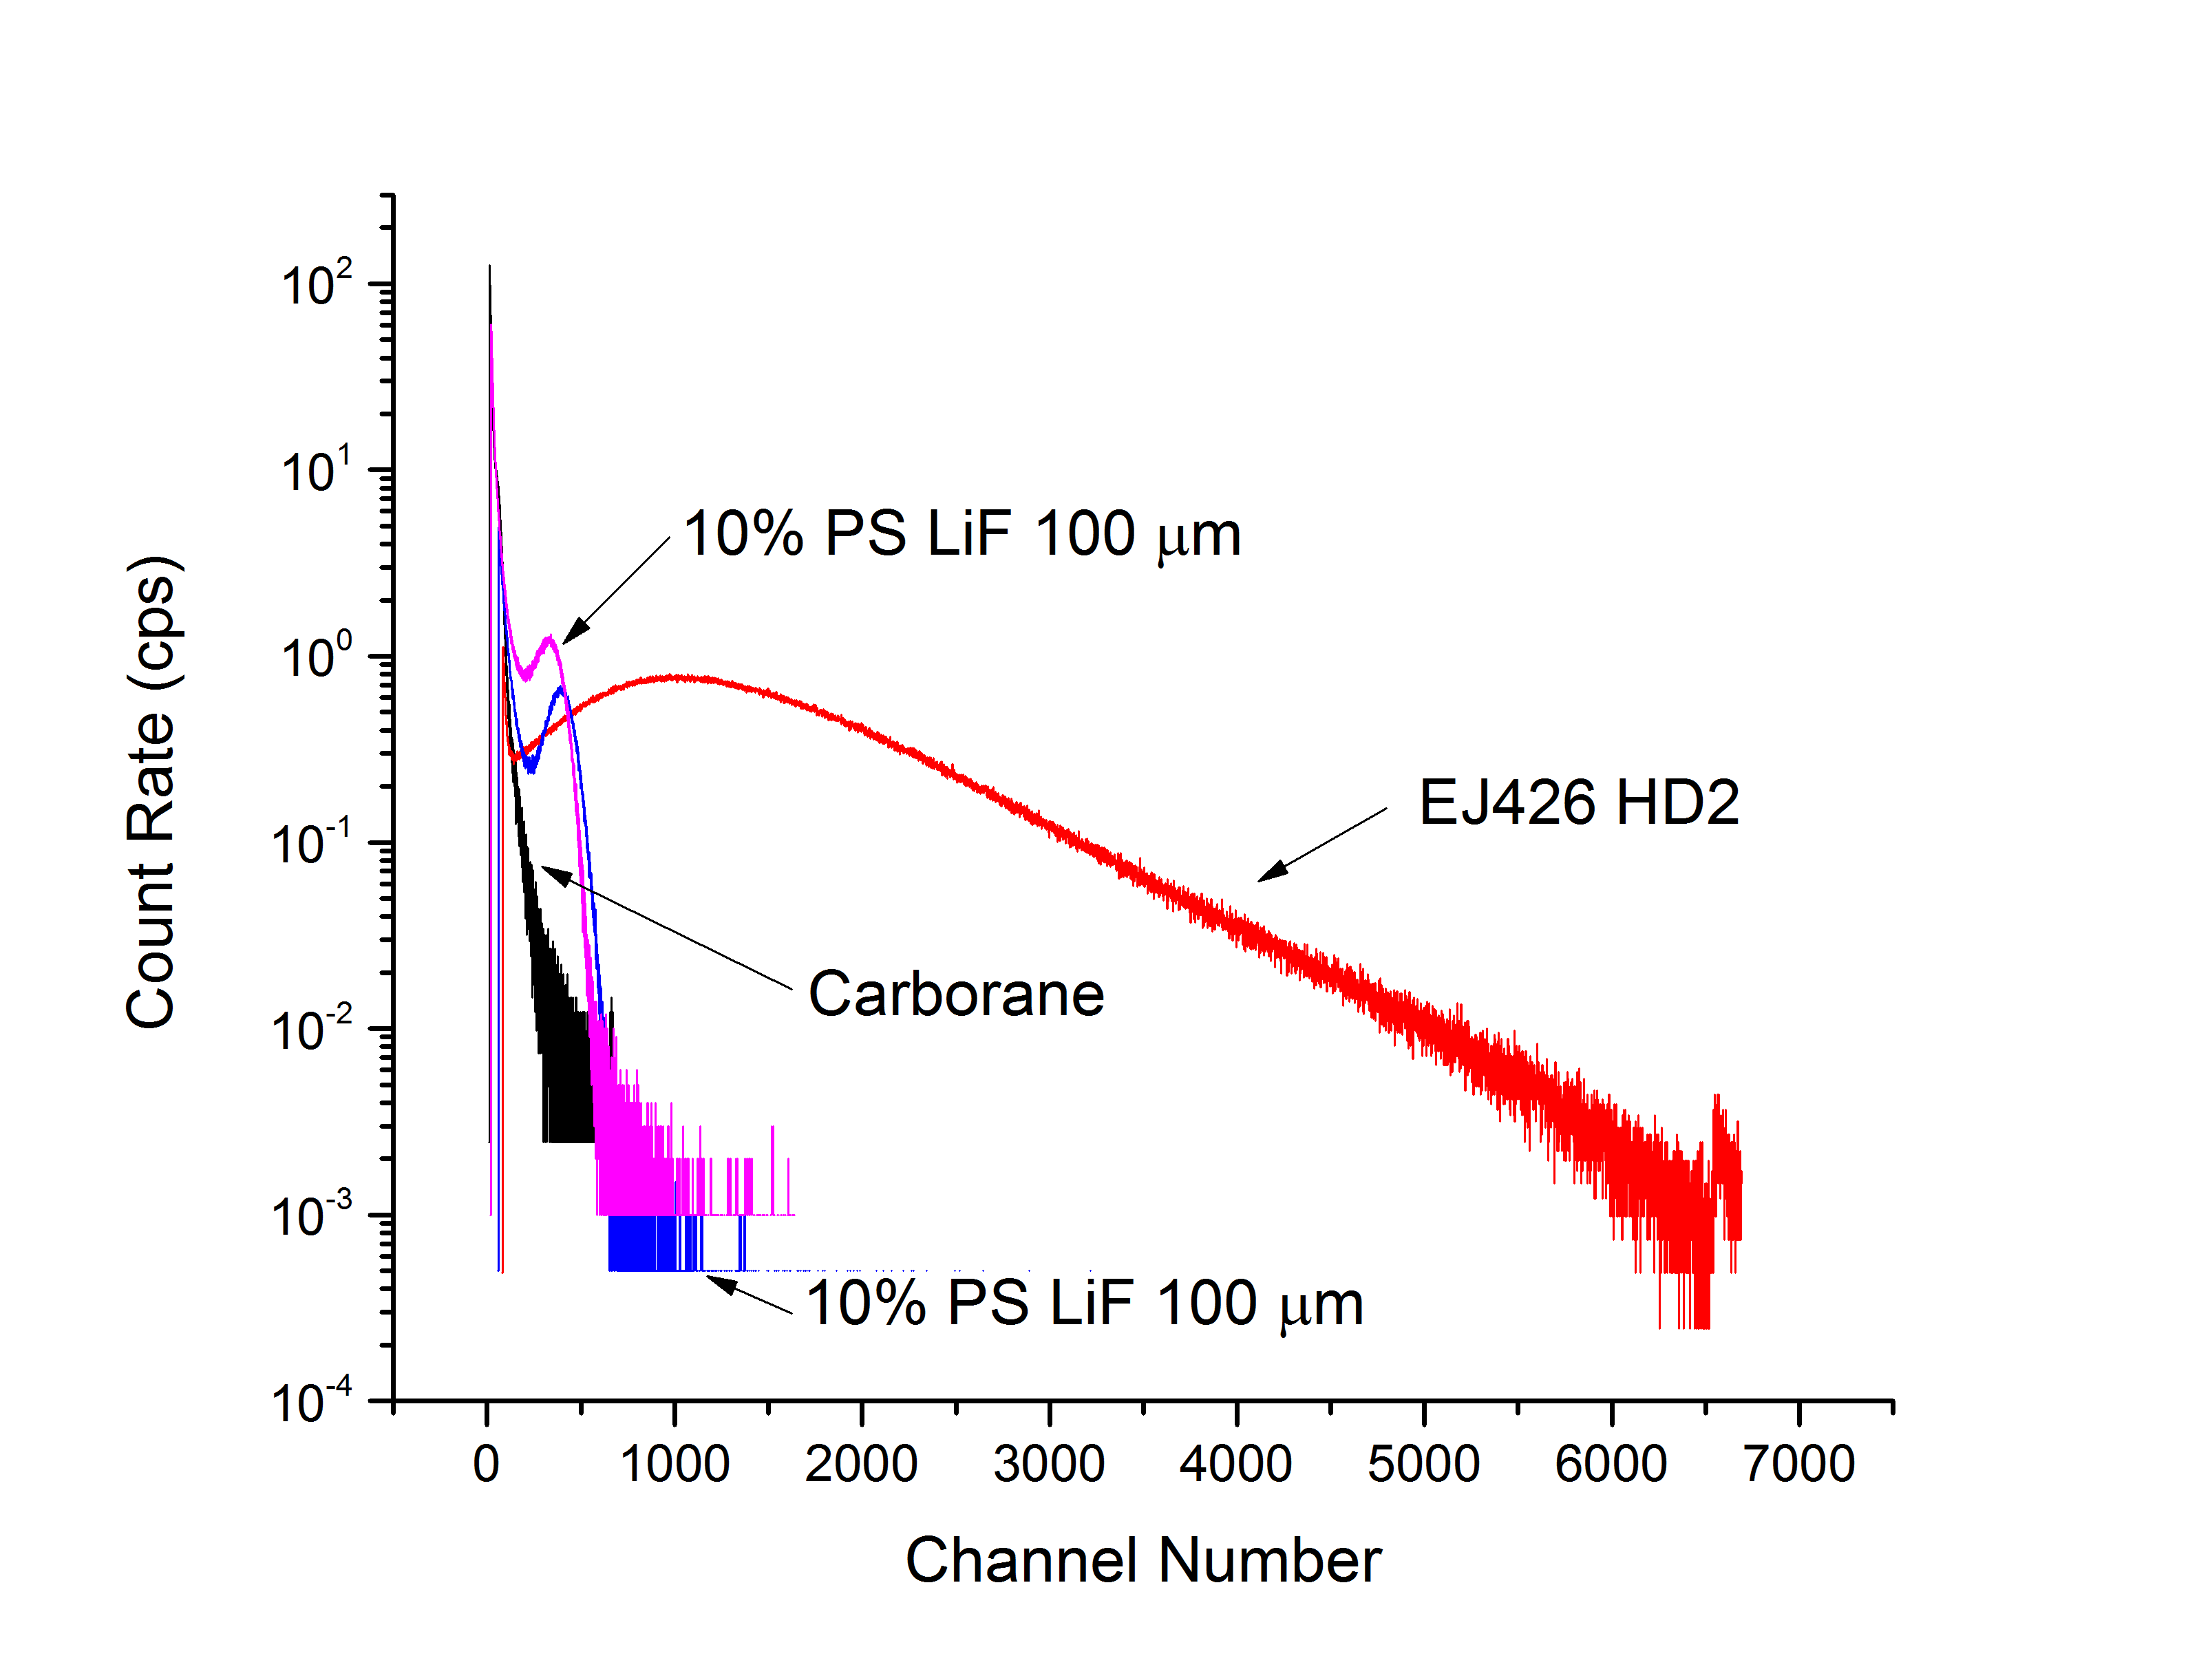
\includegraphics[width=\textwidth]{Meas_LayeredDetectorLightYield}
	\caption[Measured Light Yield of the 4" by 6" Assembiles]{Measured light yield of the 4" by 6" detector assemblies. The response of the ZnS:Ag doped with \iso[6]{LiF} dominated the response.  The effect of a doubling the thickenss of the polystyrene films is observed in the higher count rate of the \SI{100}{\um} film with a slightly lower light yield than the \SI{50}{\um} film.}
	\label{fig:4by6MeasSpectra}
\end{figure}
